
\documentclass[twocolumn]{article}

%%%%%%%%%%%%%%%%%%%%%%%%%%%%%%%%%%%%%%%%%%%%%%%
%% Comment / uncomment for one or two column(s) fomat
%\documentclass{article}

\usepackage[modulo,switch]{lineno}
\modulolinenumbers[1]
%%%%%%%%%%%%%%%%%%%%%%%%%%%%%%%%%%%%%%%%%%%%%%%
%% Comment / uncomment for showing line numbers
\linenumbers

\usepackage[latin9]{inputenc}
\usepackage{amsmath}
\usepackage{amssymb}
\usepackage{graphicx}

\makeatletter\@ifundefined{date}{}{\date{}}
\makeatother

\markright{\hfill Gontier {\em et al.}, p.\ }
\pagestyle{myheadings}

\paperheight297mm \paperwidth210mm
\textwidth170mm  \textheight245mm  \oddsidemargin 20mm
\evensidemargin\oddsidemargin \hoffset-22.4mm \voffset-28.4mm
\topmargin0pt \headheight20mm \headsep4mm \topskip0mm
\footskip17.5mm \columnsep7mm \arraycolsep2pt \parindent10pt
\renewcommand{\abstractname}{Summary}


\usepackage[english]{babel}
\usepackage[T1]{fontenc}

\usepackage{amsmath}
\usepackage{amsfonts}
\usepackage{amssymb}
\usepackage{fancyhdr}
\usepackage[hidelinks]{hyperref}
\usepackage{graphicx}
\usepackage{epstopdf}
\usepackage{pdflscape}
\usepackage{multirow}
\usepackage{subcaption}
\usepackage{bbm}
\usepackage{color}
\DeclareMathOperator*{\argmax}{arg\,max}
\newcommand{\ml}[1]{\textcolor{red}{ML : #1}}
\begin{document}
\author{F\'elix Gontier $^1$, Catherine Lavandier $^2$, Pierre Aumond $^{2, 3}$\\Mathieu Lagrange $^1$, Jean-Francois Petiot $^1$}
\date{
$^1$ LS2N, UMR CNRS 6004, Ecole Centrale de Nantes, F-44321, France\\
$^2$ ETIS, UMR CNRS 8051, University of Paris Seine, University of Cergy-Pontoise, ENSEA, CNRS, F-95000, France\\
$^3$ IFSTTAR, CEREMA, UMRAE, F-44344, Bouguenais, France
}
\title{Estimation of the perceived time of presence of sources in urban acoustic environments using deep learning techniques}
\maketitle


\begin{abstract}
The impact of urban sound on human beings has often been studied from a negative point of view (sound pollution), but in the two last decades with the soundscape approach, the positive impact has been revealed (resourcing spaces). The literature shows that the recognition of sources plays a great role in the way humans are affected by sound environments. There is thus a need for characterizing urban acoustic environments not only with sound pressure measurements but also with source-specific attributes such as their perceived time of presence. Combined, they allow the prediction of important affective dimensions of the soundscape such as its pleasantness. However, computationally predicting source-specific attributes from recordings of sensors is notably harder than computing sound pressure levels.

This paper demonstrates, on a controlled dataset, that machine learning techniques based on state of the art neural architectures can predict the perceived time of presence of several sound sources with excellent performance, at a degree of precision that is sufficient to predict perceived pleasantness. To do so, a corpus of simulated sound scenes is first designed. Perceptual attributes corresponding to those stimuli are gathered through a listening experiment. The availability of the contributions of the individual sound sources within the simulated sound scenes then allows the training and validate the proposed estimation procedure.

PACS numbers: 43.66.Lj (Perceptual effects of sound), 43.60.-c (Acoustic signal processing)
\end{abstract}


\section{Introduction}
\label{sec:intro}
In urban areas, the decrease of quality of sound environments resulting from urbanization is a major cause of annoyance, and has been identified as an important health factor. Consequently, the 2002/49/CE European directive~\cite{ec2002} requires the development of noise maps in large cities. These maps aim at providing useful tools for urban planning and noise reduction purposes. As an alternative to the noise-only paradigm, the soundscape approach defined in the ISO 12913-1~\cite{iso2014} norm as "the acoustic environment as perceived and understood and/or experienced by people and/or society, in context" extends the characterization of sound environments by considering the possible positive influence of some of its components.

The assessment of soundscape quality through standardized perceptual descriptors has been extensively studied~\cite{viollon2000, axelsson2010, cain2013, jeon2018, aletta2016}. Aletta et al.~\cite{aletta2016} did a review of soundscape descriptors and conclude that the potential soundscape descriptors identified so far seem to converge towards a two-dimensional soundscape model of perceived affective quality where one dimension corresponds to the pleasantness of the soundscape, and the orthogonal one corresponds to its enventfulness~\cite{axelsson2010, aumond2017, delaitre2014}. In this paper, we will focus on the first affective dimension which is pleasantness. Pleasantness is mainly linked to the perceived loudness~\cite{blauert1997, jekosch2004} but it also depends on the activity of sources of interest~\cite{nilsson2007, perez2012}. While the exact taxonomy of sources used differs across studies~\cite{guastavino2007, gygi2007, salamon2014, brown2011}, three major source types are found to contribute to pleasantness in urban contexts: technological, human and natural sources~\cite{nilsson2007, axelsson2010} where traffic noise, human voices and birds calls can respectively be used as a proxy of these three types~\cite{lavandier2006, ricciardi2014, aumond2017}. In existing models, source activity can be quantified by the dominance~\cite{hong2017}, the emergence~\cite{guastavino2006} or the time of presence~\cite{ricciardi2014}. However, the perceptual characterization of soundscapes requires subjective inputs, and thus cannot directly be applied to the production of perceptually motivated noise maps.

Leveraging the advent of the Internet of Things (IoT) and the availability of low-cost sensor networks~\cite{ardouin2018, mydlarz2017} could allow us to predict pleasantness or other perceptual factors from acoustic measurements at a reasonable cost. Though, bridging the gap between raw data issued from the sensors to reasonable estimates of perceptual attributes is yet an ongoing area of research. Ricciardi et al.~\cite{ricciardi2014} present a physical model of pleasantness using the variations of the measured sound level only. Because these indicators are not representative of the composition of the sound scene, the model underperforms when compared to the predictions computed using perceptual assessments. Aumond et al.~\cite{aumond2017} explore new indicators based on spectral and temporal variations in recordings of sound scenes. These indicators are designed to model the activity of specific sound sources, specifically human voices and birds, but their discriminative properties are limited. In order to tackle this issue, the recent advances in machine learning can be useful to better approximate the contributions of sound sources relevant for perceptual attribute prediction such as pleasantness.

In this paper, we do so by developing new indicators relying on source recognition models based on deep learning techniques, which is a growing interest in the machine listening community~\cite{cakir2015, salamon2017-2}. Large amounts of data with task-specific annotations are needed for these architectures to learn to extract relevant information from recordings. To the best of our knowledge such databases do not currently exist in the literature in the case of source recognition with perceptual activity labels. We propose in this paper to study the potential of the use of simulated corpora~\cite{lafay2016, salamon2017} for such purpose.

More precisely, the contributions of this paper are three-fold:
\begin{enumerate}
  \item Provide a corpus of simulated scenes for which relevant acoustic properties are well controlled and perceptual judgements are available\footnote{Corpus available at \url{https://zenodo.org/record/3248734\#.XQjC4v7gqUk}}.
  \item Propose numerical means\footnote{Open source code is available at \url{https://github.com/felixgontier/soundSourcePresenceEstimation}.} for predicting the perceived time of presence of sound sources from raw acoustic data using deep learning approaches, with a larger corpus of simulated scenes\footnote{Corpus available at \url{https://zenodo.org/record/3248703\#.XQjDVv7gqUk}}.
  \item Demonstrate through a comparative study with state of the art approaches that the proposed method allows the prediction of pleasantness to a sufficient degree of accuracy.
\end{enumerate}

First, a perceptual test is conducted in Section~\ref{sec:data} where simulated sound scenes are compared to recordings in order to validate the relevance of the proposed protocol for \textit{in situ} sound environments. Section~\ref{sec:methods} presents the design of a deep learning architecture that performs multi-label sound source recognition at relevant time scales. Time of presence estimations from this architecture are evaluated in Section~\ref{sec:results} in the context of pleasantness prediction, in comparison to existing models from perceptual and physical indicators.

\section{Perception of simulated sound scenes}
\label{sec:data}

\subsection{Corpus generation}
\label{sec:data_corp}

A corpus is first created to validate the use of simulated sound scenes in the development of time presence prediction models. It is based on recordings from one of the four soundwalks performed in~\cite{aumond2017}, including 19 locations in the 13th district of Paris, France. A classification of these scenes is proposed in~\cite{gloaguen2017} in terms of ambiance: \textit{park}, \textit{quiet street}, \textit{noisy street} and \textit{very noisy street}. For each of the 19 recordings, 45 seconds of audio in a single channel are extracted. This duration is chosen to be perceptually relevant for the perceptual evaluation of sound environments. The 45~s segments are selected to represent the properties of their respective ambiances in terms of source composition, without single events overwhelming their overall perception. The extracts are then subjectively annotated in terms of the following properties:

\begin{itemize}
\item Background sources that are present throughout the whole scene, and their respective sound level considered constant,
\item Sound events characterized for each occurrence by their source type, onset-offset and event-to-background ratio (EBR) in dB.
\end{itemize}

The 45~s sound scenes are then replicated using the  \textit{simScene} software, an open source software library in Matlab that allows the simulation of sound scenes as the additive composition of sound sources, using a database of recordings associated to these sources\footnote{\url{https://bitbucket.org/mlagrange/simscene}}. Here the database is constructed from excerpts of the LibriSpeech~\cite{panayotov2015} corpus for voices and Freesound\footnote{\url{https://freesound.org}} contributions for remaining sources. The original recordings from 6 locations (P1, P3, P4, P8, P15 and P18) are chosen for perceptual comparison, as they explore diverse real-life situations with respect to environment categorization. The 6 recorded and 19 replicated scenes are normalized so that their playback sound level through the restitution system is the same as measured during recording, with a range from 63.9~dB SPL to 79.4~dB SPL.


\begin{figure*}[th]
    \centering
     \begin{subfigure}[t]{0.33\textwidth}
        \centering
        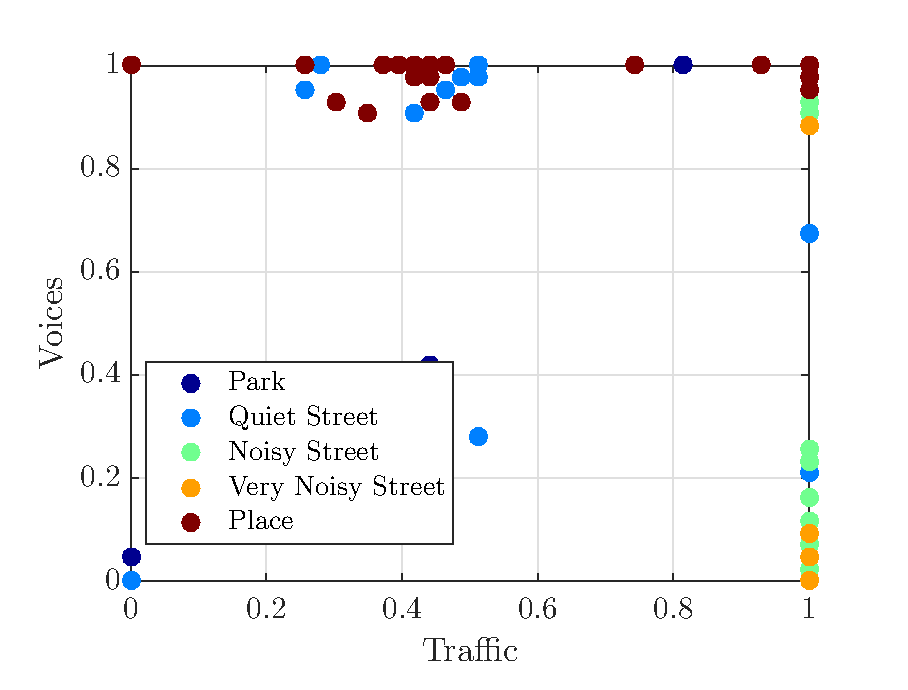
\includegraphics[width=\textwidth]{figures/tv_pres.eps}
    \end{subfigure}%
    \begin{subfigure}[t]{0.33\textwidth}
        \centering
        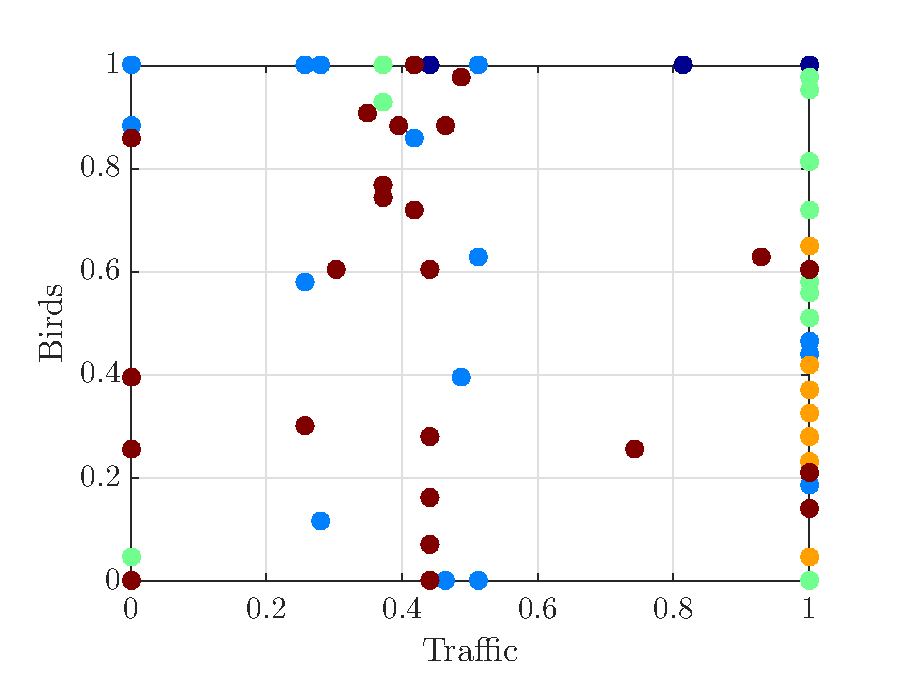
\includegraphics[width=\textwidth]{figures/tb_pres.eps}
    \end{subfigure}
    \begin{subfigure}[t]{0.33\textwidth}
        \centering
        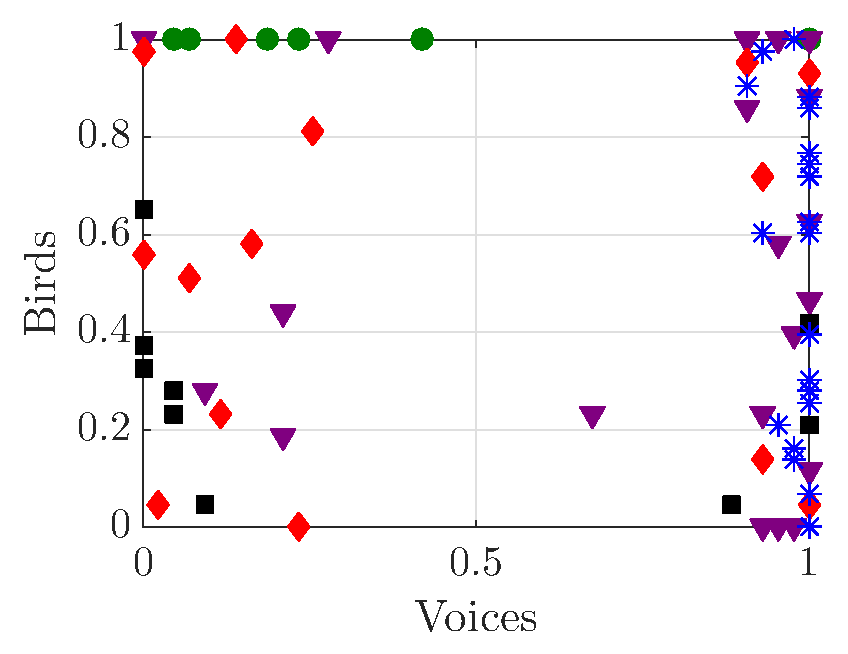
\includegraphics[width=\textwidth]{figures/vb_pres.eps}
    \end{subfigure}
    \caption{Physical estimations~\cite{gontier2018} of the perceived time of presence of traffic, voices and birds sources for the corpus of simulated scenes with automatically generated scenarios.}\label{fig:tvb_pres}
\end{figure*}

To further study the perceptual properties of simulated scenes, the corpus is extended with 75 simulated scenes corresponding to new scenarios. Previous studies show that pleasantness is mainly influenced by the activity of three sources: \textit{traffic}, \textit{human voices} and \textit{birds}. We choose to restrict the scene composition to these 3 sources. Newly generated scenarios should cover most real-life situations while remaining perceptually plausible. To do so, statistics on background and event properties are extracted for each of the three sources from annotations presented in~\cite{gloaguen2017}. These statistics include, conditionally to the ambiance (resp. \textit{park}, \textit{quiet street}, \textit{noisy street}, \textit{very noisy street} and \textit{square}):

\begin{itemize}
\item The probability of appearance of a given source in the scene, for which events and backgrounds are considered separately,
\item Event-to-background ratios (EBR) in dB for all events and backgrounds compared to a main background source, drawn from gaussian distributions with parameters identified from annotations of recordings,
\item The inter-onset of event occurrences in seconds, also drawn from gaussian distributions.
\end{itemize}

Adjustments are made on the variance of the considered properties to better cover possible scenarios. Since voice events consist mostly of read English recordings, their EBR is reduced to improve realism. An additional \textit{square} ambiance is added with properties derived empirically from available data. Diverse new scenarios are then generated by sampling the background and event properties distributions, resulting in 40 scenes per ambiance for a total of 200 scenes. For each scene the perceptual time of presence for the traffic, voice and bird sources is estimated using the indicators proposed in~\cite{gontier2018}. Ideally, sound scenes should cover the resulting 3-dimensional space in a homogeneous way. To do so, the 75 scenes that maximize the minimum pairwise distance in the 3-dimensional space are selected, as shown in Figure~\ref{fig:tvb_pres}. The playback sound level is also conditioned to the ambiance according to typical sound levels in urban context, and ranges from 46.6~dB SPL to 77.1~dB SPL.

The experiment corpus thus totals 100 scenes: 6 recorded, 19 replicated scenes from the Grafic project, and 75 simulated scenes.


\subsection{Perceptual experiment}
\label{sec:data_exp}

In order to gather estimates of the perceptual attributes and to validate the usefulness of the proposed corpus, a perceptual experiment is conducted. Participants are asked to evaluate sound scenes in terms of 9 criteria represented by 11 point scales (0-10). These scales are presented in French and translated in this report using standard terminology. The first 5 scales relate to general properties of the scene:
\begin{itemize}
\item Pleasantness: \textit{Unpleasant - Pleasant} (\textit{D\'esagr\'eable - Agr\'eable}) - P,
\item Liveliness: \textit{Inert, amorphous - Lively, eventful} (\textit{Inerte, amorphe - Anim\'e, mouvement\'e}) - L,
\item Overall loudness: \textit{Quiet - Noisy} (\textit{Silencieux - Bruyant}) - OL,
\item Interest: \textit{Boring, uninteresting - Stimulating, interesting} (\textit{Ennuyeux, inint\'eressant - Stimulant, int\'eressant}) - I,
\item Calmness: \textit{Agitated, chaotic - Calm, peaceful} (\textit{Agit\'e, chaotique - Calme, tranquille}) - C.
\end{itemize}

These quantities are typically studied in the perceptual characterization of sound scenes~\cite{axelsson2010, aumond2017, nilsson2007}. While this work focuses on the application of pleasantness prediction, including other dimensions can be useful to verify the relevance of simulated data in relation to previous work on real scenarios.

The perception of source activity can be linked to the notions of dominance, time of presence, or emergence. The perceptual time of presence, that is the percentage of time for which the corresponding source is heard, is selected as the activity descriptor for this study. The influence of traffic on pleasantness is further separated into that of background and salient events. Thus, 4 additional questions are presented to the participants and evaluated on the same 11 point scales:
\begin{itemize}
\item Sound level of passing vehicles: \textit{Very low - Very high} (\textit{Tr\`es faible - Tr\`es fort}) - $L_{T, p}$,
\item Time of presence of Traffic, Voices, Birds: \textit{Never - Continuously} (\textit{Jamais - Continuellement}) - resp. $T_{T, p}$, $T_{V, p}$ and $T_{B, p}$
\end{itemize}
where $p$ denotes a perceptual evaluation.

Prior to the test, a short verbal introduction is given to the participants and the interface is introduced to ensure that the quantities are well understood. Although the corpus is comprised of 100 sound scenes, participants only evaluate 50 scenes: all listen to the 6 recorded and 19 replicated sound scenes, then to 25 of the 75 simulated with new scenarios according to a balanced incomplete block design~\cite{dagnelie2003}. The selection of simulated scenes is done so that all scenes in the sub-corpus are evaluated by the same number of participants. All participants are first presented with the most quiet then loudest of the recorded scenes (resp. P3 and P15). A random listening order is generated for each subject to control ordering effects for the remaining of the test. Participants can listen to each scene once, and have to listen to the full extract and to answer all questions before being allowed to proceed to the next scene.

The scenes are played at a given sound level as discussed in Section~\ref{sec:data_corp}, through the same computer and sound card configurations. Beyerdynamics DT-990 Pro headphones are used by all participants. These headphones are calibrated in a semi-anechoic chamber where a relation between the playback sound level and the sound card output voltage is obtained for pink noise. From this information a scaling factor is applied to the sound scenes to ensure that they are heard at the desired sound level by every listener.

A total of 23 students aged from 22 to 23 years including 16 males and 7 females at Ecole Centrale de Nantes completed the test (note that with 23 subjects, the incomplete block design is not perfectly balanced). All gave consent prior to the experiment and reported normal hearing.

\subsection{Corpus validation}
\label{sec:data_val}

The perceptual responses of the 6 recorded and corresponding replicated scenes are first studied. Table~\ref{tab:ogrep} shows the mean differences between assessments for pairs of scenes with equivalent scenarios. Wilcoxon signed-rank tests~\cite{wilcoxon1945} are implemented for each scene and perceptual scale to outline significant differences between assessment distributions, which are shown in bold. As the data is discretely distributed, zero differences between paired samples are included using Pratt's modification of the test~\cite{pratt1959}. On the first five scales, all mean differences are lower than 2 points on the 11-point Likert scale. Though, significant differences are outlined that can be linked to corresponding discrepancies in source-specific parameters. The highest difference (-5.22) is found for the assessment of the time of presence of traffic in the location P4. For this location, the background traffic in the recorded scene varies along time, it is louder in the first half of the scene than in the second half. Replicating this scene using simScene imposes a constant sound level for background sources. Thus, the background traffic is louder in the replicated scene than it is in the recording for about half of its duration. To a lesser extent the same issue explains the large difference (-4) in the assessed time of presence of voices in the location P3. Discrepancies on source-specific scales can also be interpreted by the choice of isolated samples, which is semi-random and based on a high-level source taxonomy. For example, no difference is made during annotation between child or adult speech, or depending on its expressiveness. Though, overall no consistent difference between the perception of recorded and replicated scenes emerges for the studied points.

\begin{table*}[t]
\centering
\caption{Mean differences of perceptual assessments between original and replicated sound scenes. Significant differences as per a Wilcoxon signed-rank test are shown in bold (n=23, p<0.05)}
\label{tab:ogrep}
%\resizebox{\columnwidth}{!}{
\begin{tabular}{ c | c c c c c c c c c }
\hline
	 & P & L & OL & I & C & $L_{T, p}$ & $T_{T, p}$ & $T_{V, p}$ & $T_{B, p}$ \\ \hline
	P1 & 0.43 & \textbf{-1.65} & \textbf{-1.04} & 0.43 & 0.13 & \textbf{-0.91} & 0.39 & \textbf{-2.09} & 0.61 \\
	P3 & 0.26 & -0.43 & 0.30 & -1 & 0.30 & 0.35 & 1.04 & \textbf{-4} & 0.22 \\
	P4 & 0.91 & 0 & \textbf{-1.83} & 0.48 & \textbf{1.30} & \textbf{-0.96} & \textbf{-5.22} & \textbf{1.43} & 0.04 \\
	P8 & 0.26 & \textbf{-1.65} & -0.87 & -0.96 & 0.65 & \textbf{-2.04} & \textbf{-0.91} & 0.09 & \textbf{-1.43} \\
	P15 & \textbf{-1.35} & 0.52 & 0.52 & \textbf{-1.17} & 0.09 & 0.61 & 0.13 & \textbf{1.96} & \textbf{-2.74} \\
	P18 & \textbf{1.13} & -0.30 & \textbf{-1.17} & -0.43 & \textbf{1.39} & -1.04 & \textbf{-1.83} & \textbf{0.83} & \textbf{1.30} \\ \hline
\end{tabular}
%}
\end{table*}

Next, the perceptual space generated by the experiment's five general scales (P, L, OL, I and C) is studied to validate the use of simulated sound scenes with new scenarios as well as reduced source complexity. It is obtained by performing a principal components analysis (PCA) on the corresponding perceptual responses averaged along participants. No standardization is applied to the data. Figure~\ref{fig:pspace_rec} and Figure~\ref{fig:pspace_sim} compare the results for scenes based on recordings (n=25) and new scenarios (n=75) respectively. The resulting spaces are similar, with only overall loudness and pleasantness axes slightly rotated between the two subcorpora. For both sets the variance explained by the first two components is similar, resp. 79.4\% - 18.1\% and 79.6\% - 15.2\%. Furthermore, these representations are comparable to those found in previous work on perceptual dimensions~\cite{axelsson2010, cain2013}. Thus, the use of simulated scenes based on both real and new scenarios does not result in major differences in the relations between perceptual quantities. Additionally, the assessments averaged on all subjects are projected onto the PCA space for each scene and represented in Figure~\ref{fig:pspace_sim} as dots for simulated scenes corpus and crosses for recorded and replicated scenes. These projections show that the space covered by scenes based on new scenarios covers that of the studied real-life environments. This further demonstrates the effectiveness of the scene generation procedure in terms of diversity of scenarios.

Discrepancies between projections of original and replicated scenes are highlighted in Figure~\ref{fig:pspace_rec} using arrows. The standard deviation of assessments is represented using ellipses for one location (P1). The projections of assessment distributions consistently overlap for all pairs of recorded and replicated scenes\footnote{Data available here \url{http://felixgontier.github.io/soundSourcePresenceEstimation/web/index.html}}. This illustrates the results in Table~\ref{tab:ogrep} where perceptual assessments were not found to differ significantly overall.

\begin{figure}[th]
    \centering
    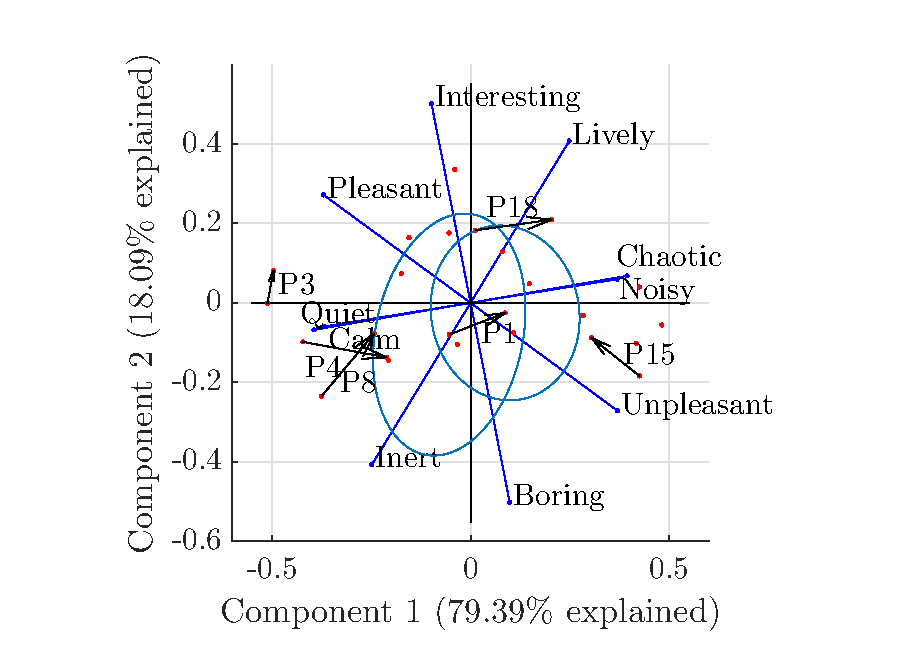
\includegraphics[width=0.8\columnwidth]{figures/pca_p1.eps}
    \caption{Biplot of the principal components analysis of average assessments for the 5 general questions on the 6 recorded and 19 replicated scenes (n=25). Arrows show discrepancies between corresponding recorded and replicated scenes. For the P1 recording location the standard deviation of the projection of individual responses is shown using ellipses.}\label{fig:pspace_rec}
\end{figure}
\begin{figure}[h]
    \centering
    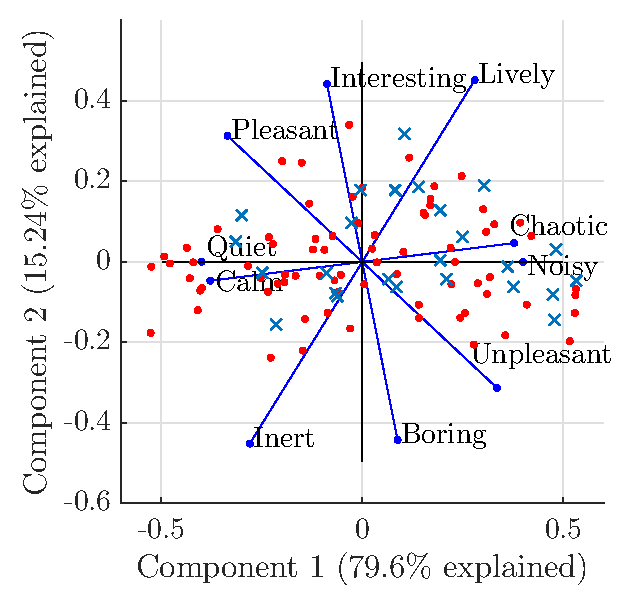
\includegraphics[width=0.8\columnwidth]{figures/pca_sim.eps}
    \caption{Biplot of the principal components analysis of average assessments for the 5 general questions on the 75 simulated scenes (n=75). Assessments of simulated scenes are projected as dots, and recorded and replicated scenes are projected as crosses.}\label{fig:pspace_sim}
\end{figure}


\section{Methods}
\label{sec:methods}

\subsection{Acoustical indicators for soundscape description}
\label{sec:methods_inds}

Based on previous studies~\cite{aumond2017, gontier2018, ricciardi2014}, several indicators are identified that correlate well with perceptual parameters. These indicators can be used to develop baseline physical models of pleasantness in the design of a deep learning architecture for sound source recognition.

First, indicators can be computed directly from the mixed audio, without the need for information about the composition of the scene, \textit{i.e.} source activity and level. Typically this includes indicators derived from sound level measurements. For this study the following variables are computed with a time frame of 1~s using the Matlab ITA-toolbox~\cite{itatoolbox2017}:

\begin{itemize}
\item Z-weighted $L_{eq}$ and A-weighted $LA_{eq}$ equivalent sound levels in dB and dBA respectively.
\item $L_{10}$, $L_{50}$ and $L_{90}$: 10th, 50th and 90th percentiles of the Z-weighted sound level. The $L_{10}$ is often associated to events and the $L_{90}$ to background activity, while the $L_{50}$ is a measurement of the overall sound level.
\item $LA_{50}$: 50th percentile of the A-weighted sound level, with similar properties as the $L_{50}$.
\item $L_{50, 1kHz}$: 50th percentile of the Z-weighted sound level for the 1kHz frequency band, also a good descriptor of the overall sound level of the scene.
\item $LA_{10}-LA_{90}$: Emergence indicator included in the pleasantness model presented in~\cite{ricciardi2014}.
\end{itemize}

The time and frequency second derivative ($TFSD$) is introduced in~\cite{aumond2017} as a descriptor of source activity. Its expression is:

\begin{equation}
TFSD_{f, t} = \frac{\lvert\frac{d^2L(f, t)}{dfdt}\rvert}{\sum_{f1=31.5Hz}^{f1=16kHz}\lvert\frac{d^2L(f1, t)}{df1dt}\rvert}
\end{equation}
where $L(f, t)$ is the third-octave spectrum of the signal. To provide a baseline for pleasantness prediction, the $TFSD$ is computed for the 4kHz band and 125ms measurements ($TFSD_{4kHz(1/8s)}$), and for the 500Hz band with 1s measurements ($TFSD_{500Hz, 1s}$) as estimates of the contribution of birds and voices respectively.

The simulation process of the scenes outputs ground truth source contributions as separate channels. Additional indicators are computed on the separated audio signals for the traffic, voices and birds sources: The equivalent sound level $L_{eq, s}$ for source $s$ and the source emergence $\Delta L_{s}$, taken as the difference between the equivalent sound level of source $s$ and that of all other sources combined.

Next, the $\hat T_s(\alpha, \beta)$ time of presence approximation proposed in~\cite{gontier2018} is computed. $\hat T_s(\alpha, \beta)$ is based on a binary source emergence model computed on the third-octave band emergence spectrum $\Delta L_{s}(t, f)$. It is parametrized by $\alpha$ and $\beta$ thresholds:

\begin{align}
\hat T_s(\alpha, \beta) &= \frac{1}{N_t}\sum_{t = 1}^{N_t}\mathbbm{1}\left[ \frac{\sum_{f = 1}^{N_f}\Delta L_{s}(t, f)\mathbbm{1}_{\Delta L_{s}(t, f)>\alpha}}{\sum_{f = 1}^{N_f}\mathbbm{1}_{\Delta L_{s}(t, f)>\alpha}}>\beta \right]\\
\alpha_{opt},\beta_{opt} &= \argmax_{\alpha, \beta}\frac{1}{N_s}\sum_{s = 1}^{N_s}r\left(T_{s, p}, \hat T_s(\alpha, \beta)\right)
\end{align}

where $r$ is the Pearson's correlation coefficient, $s$ denotes the sound source, $N_s$ is the number of sources in the taxonomy and equals 3 in this study, $t$ is the time frame and $T_{s, p}$ corresponds to the perceptual time of presence assessments averaged per scene. This indicator evaluates the presence or absence of a given source in a small time frame. First, frequency bands for which the source is emergent by more than the $\alpha$ threshold value are isolated. Then, the source is considered present if the emergence for these bands is on average greater than the $\beta$ threshold. A time of presence estimation is obtained for each source by averaging along the $N_t$ time frames composing the scene. The optimal threshold values are optimized once in this study on the whole perceptual experiment corpus, and found as $\alpha_{opt} = -14dB$ and $\beta_{opt} = -7dB$.

In the remainder of this paper, the subscript $s$ is replaced with the corresponding source initial: $T$ for traffic, $V$ for voices and $B$ for birds.


\subsection{Source presence detection using deep learning}
\label{sec:methods_deep}

Considering machine learning techniques to detect the presence of source requires the availability of annotated data. Thus, in order to train deep learning architectures for source recognition, a larger corpus is constructed. It is composed of two datasets of simulated scenes:
\begin{itemize}
\item The development set, made of 400 scenes of 45~s each (total duration 5 hours), which is used during the training process,
\item The evaluation set, made of 200 scenes of 45~s each (total of 2.5 hours), which is used to compute the performance of the trained model and its generalization capabilities.
\end{itemize}

The generation procedure is the same for both datasets, and is equivalent to that of the 75 scenes in the simulated sub-corpus considered for the perceptual test in Section~\ref{sec:data_corp}. Only traffic, human voices and birds sources compose the sound scenes. To generate the scenes, it is important to ensure a complete independance of the training and test set. For that, the isolated samples database is split in the same proportions as the two datasets: two-thirds for the development set and the remaining one-third for the evaluation set. As a result, while the generation process is the same for both corpora, the scenarios and audio samples are different.

The developped model should extract relevant source information from a representation of the audio signal. Typically, spectral representations such as mel bands are preferred to the raw audio waveform because of the regularities they underline in the signal. Here, the third-octave spectrum is considered as it is commonly used in acoustic monitoring applications~\cite{ardouin2018, gontier2017}. Third-octave spectra are computed for 125~ms frames and 29 frequency bands in the $20~Hz - 12.5~kHz$ range. Inputs are then obtained by splitting the resulting spectrograms into texture windows of 1~s duration, which is considered a relevant scale for perception. The spectral blocks of dimension 29x8 are then processed independently in this study.

Target outputs are associated to each input frame to train the model. In~\cite{gontier2018} the time of presence of traffic, voices and birds was successfully approximated by the $\hat T_s(\alpha, \beta)$ indicator. Thus, the source presence values given by this indicator can be used as weak perceptual time of presence labels. Alternatively, it is possible to perform sound level estimation using ground truth labels provided by the simulation process before computing $\hat T_s(\alpha_{opt}, \beta_{opt})$.

A deep learning model is implemented and trained for the source presence prediction task, with the architecture shown in Figure~\ref{fig:deep_arch}. The model includes 4 blocks of convolutional layers followed by leaky rectified linear unit (LeakyReLU) activations of expression $y = max(0.1x, x)$. The convolutional layers have respectively 128, 64, 32 and 32 output channels, and a common kernel size of 5x5. The output of the last block is flattened then goes through a fully connected layer with output size 3. A final sigmoid activation is used in order to obtain outputs in the 0-1 range, which correspond to the presence of traffic, voices and birds in the 1~s frame respectively. During training these values are directly compared to presence labels given by $\hat T_s(\alpha_{opt}, \beta_{opt})$ using a binary cross-entropy cost function:

\begin{equation}
BCE(y, \hat y) = -\sum_s y_s log\left(\hat y_s\right) + (1-y_s) log\left(1-\hat y_s\right)
\end{equation}
where $s$ is the source, $y_s$ and $\hat y_s$ are the target and predicted presence for source $s$ in the 0-1 range. This loss function is minimized using the Adam algorithm~\cite{kingma2015} on batches of 1~s examples. During evaluation, a threshold of 0.5 is independently applied to the 3 outputs to obtain a binary presence value for each source: each source is considered absent when the model outputs a value lower than 0.5 and present when it outputs 0.5 or higher. The time of presence estimation is then obtained by averaging presence labels of all 1~s time frames corresponding to the same scene.

\begin{figure}[t]
    \centering
    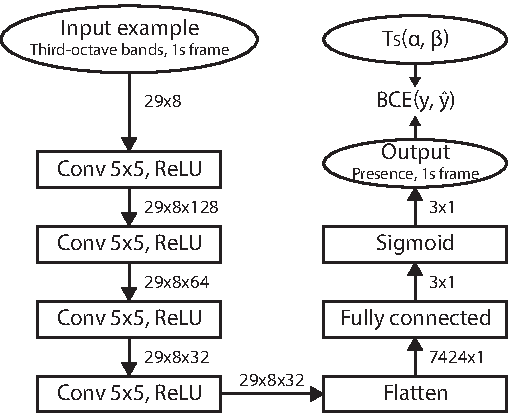
\includegraphics[width=\columnwidth]{figures/deep_arch.pdf}
    \caption{Architecture of the deep learning model used for source presence prediction.}\label{fig:deep_arch}
\end{figure}

\section{Results}
\label{sec:results}

The proposed method for predicting the time of presence of sources is evaluated in the context of pleasantness estimation. To this aim, baseline models are first constructed using data from the experiment in Section~\ref{sec:data_exp} and from previous work.

\subsection{Perceptual pleasantness model}
\label{sec:results_perc}

\begin{table*}[t]
\centering
\caption{Pearson's correlation coefficients between perceptual scales at the scene level (n=100, *: p<0.05, **: p<0.01)}
\label{tab:percc}
%\resizebox{\columnwidth}{!}{
\begin{tabular}{ c | c c c c c c c c c }
\hline
	 & P & L & OL & I & C & $L_{T, p}$ & $T_{T, p}$ & $T_{V, p}$ & $T_{B, p}$ \\ \hline
	P & 1 & -0.53** & -0.89** & 0.66** & 0.88** & -0.82** & -0.76** & 0.05 & 0.57** \\
	L &  & 1 & 0.76** & 0.06 & -0.78** & 0.39** & 0.17 & 0.60** & -0.36** \\
	OL &  &  & 1 & -0.39** & -0.96** & 0.71** & 0.59** & 0.17 & -0.45** \\
	I &  &  &  & 1 & 0.35** & -0.55** & -0.67** & 0.38** & 0.48** \\
	C &  &  &  &  & 1 & -0.67** & -0.55** & -0.24* & 0.48** \\
	$L_{T, p}$ &  &  &  &  &  & 1 & 0.79** & -0.15 & -0.41** \\
	$T_{T, p}$ &  &  &  &  &  &  & 1 & -0.35** & -0.42** \\
	$T_{V, p}$ &  &  &  &  &  &  &  & 1 & -0.21* \\
	$T_{B, p}$ &  &  &  &  &  &  &  &  & 1 \\ \hline
\end{tabular}
%}
\end{table*}

We first study the relations between perceptual scales with respect to existing work. Table~\ref{tab:percc} shows the Pearson's correlation coefficients between pairs of parameters with assessments averaged for each scene (n=100). The resulting values are consistent with the literature~\cite{aumond2017, gontier2018}, both between general scales as discussed in Section~\ref{sec:data_val} and for the relations to source contributions. Indeed, pleasantness (P) is mainly influenced negatively by overall loudness (OL) and traffic and positively by birds. In previous studies a small positive contribution of voices to pleasantness was found, while no direct relation is visible from the data gathered. This can be explained by the choice of speech samples used during generation, which consist of read audiobooks extracts and thus may sound unnatural in the considered urban environments. Liveliness (L) is here negatively though weakly (r=-0.36) correlated with the presence of birds, while no significant relation was found in previous studies. However, its correlation with the presence of human voices is the strongest (r=0.60), as suggested by~\cite{axelsson2010}.

Relations between source-specific parameters are also weak with the exception of traffic being negatively correlated with birds (r=-0.42). The perceived sound level of passing vehicles $L_{T, p}$ is a potential alternative to the time of presence of traffic $T_{T, p}$, as it displays higher correlations with general scales and lower correlations with other source-specific parameters.

As a baseline, multilinear models of pleasantness are built as a function of the overall loudness (OL) and source-specific parameters ($L_{T, p}$, $T_{T, p}$, $T_{V, p}$, $T_{B, p}$) with assessments averaged for each scene (n=100). All 31 combinations of the 5 predictors are considered, but to ensure that no multi-collinearity is present between predictors a variance inflation factor (VIF) test is performed prior to each regression. Only combinations for which all predictors verify $VIF<5$ are considered valid. The best resulting models in terms of $R^2_{adj}$ with statistically significant coefficient estimates ($p<0.05$) are:

\begin{align}
\begin{split}
\hat P_{1, p} & = 8.56 - 0.63~OL - 0.20~L_{T, p} + 0.11~T_{V, p}\\
&\qquad + 0.14~T_{B, p} \label{eq:pp1}
\end{split}\\
\begin{split}
\hat P_{2, p} & = 8.99 - 0.67~OL - 0.15~T_{T, p} + 0.08~T_{V, p}\\
&\qquad + 0.12~T_{B, p} \label{eq:pp2}
\end{split}
\end{align}

Because of the collinearity between $L_{T, p}$ and $T_{T, p}$, both models have very similar formal expressions, with important negative contributions of the overall loudness and traffic activity. A small positive contribution of the time of presence of voices is also found despite no significant correlation underlined in Table~\ref{tab:percc}.

Table~\ref{tab:percm} summarizes performance metrics computed for the two models. $\hat P_{1, p}$ and $\hat P_{2, p}$ display similar estimation errors, adjusted $R^2$ and correlation to assessed pleasantness. The performance of obtained perceptual models is about 0.6 (RMSE), which is below the mean standard deviation of pleasantness assessments for this experiment (1.77).

\begin{table}[t]
\centering
\caption{Performance of perceptual models for pleasantness prediction (**: p<0.01).}
\label{tab:percm}
%\resizebox{\columnwidth}{!}{
\begin{tabular}{ c | c | c | c }
\hline
	 & $RMSE$ & $R^2_{adj}$ & $r$ \\ \hline
	$\hat P_{1, p}$ & 0.59 & 0.91 & 0.95** \\
	$\hat P_{2, p}$ & 0.61 & 0.90 & 0.95** \\ \hline
\end{tabular}
%}
\end{table}

\subsection{Physical pleasantness models}
\label{sec:results_phys}

The analysis of physical indicators presented in Section~\ref{sec:methods_inds} is done using the arithmetic mean of subjective assessments over all participants for replicated and simulated scenes. The 6 recorded scenes are excluded from the study as the ground truth source composition is unknown. Two scenes containing only one source are also excluded for implementation concerns, resulting in $n=92$ scenes.

Table~\ref{tab:physc} shows the Pearson's correlation coefficients between computed physical indicators and perceptual assessments. First, all global sound level indicators correlate well (r>0.9) with the perceived overall loudness. Regarding source-specific perceptual parameters, the $L_{eq, s}$ correlates consistently well with the $T_{s, p}$ of corresponding source (r=0.71). Conversely, the emergence $\Delta L_s$ fails to represent the perceived bird activity, and correlations are weak for other sources. The proposed estimates of the time of presence $\hat T_s(\alpha_{opt}, \beta_{opt})$ show strong correlations to their perceptual counterparts (r>0.8), though this is expected as $\alpha_{opt}$ and $\beta_{opt}$ are optimized to this aim. They also display good source discrimination properties, as no significant correlation is found between voices and birds, and perceptual assessments of traffic were correlated with those of other sources in Table~\ref{tab:percc}. They are also better predictors than the $TFSD_{500Hz, 1s}$ and $TFSD_{4kHz, 1/8s}$ indicators for voice and bird activity in this corpus. Interestingly, the perceived sound level of passing vehicles $L_{T, p}$ is best represented by the $L_{10}$. In perceptual models including the sound level of traffic events, the global $L_{10}$ may thus be a relevant predictor without the need for a source separation and level estimation algorithm.

\begin{table*}
\centering
\caption{Pearson's correlation coefficients between physical and perceptual indicators (n = 92, *: p<0.05, **: p<0.01). Non significant correlations at the 5\% threshold are noted NS.}
\label{tab:physc}
\resizebox{\textwidth}{!}{
\begin{tabular}{ c | c c c c c | c c c c }
\hline
	 & P & L & OL & I & C & $L_{T, p}$ & $T_{T, p}$ & $T_{V, p}$ & $T_{B, p}$ \\ \hline
	$LA_{eq}$ & -0.86** & 0.68** & 0.92** & -0.37** & -0.88** & 0.77** & 0.66** & NS & -0.41** \\
	$LA_{50}$ & -0.84** & 0.67** & 0.91** & -0.33** & -0.87** & 0.71** & 0.63** & NS & -0.35** \\
	$L_{eq}$ & -0.88** & 0.67** & 0.91** & -0.44** & -0.88** & 0.83** & 0.71** & NS & -0.46** \\
	$L_{10}$ & -0.87** & 0.65** & 0.90** & -0.44** & -0.86** & 0.84** & 0.71** & NS & -0.47** \\
	$L_{50}$ & -0.89** & 0.65** & 0.92** & -0.43** & -0.89** & 0.77** & 0.71** & NS & -0.44** \\
	$L_{90}$ & -0.86** & 0.68** & 0.92** & -0.39** & -0.89** & 0.71** & 0.67** & NS & -0.40** \\
	$L_{50, 1kHz}$ & -0.88** & 0.69** & 0.92** & -0.42** & -0.89** & 0.74** & 0.73** & NS & -0.50** \\
	$L_{10}-L_{90}$ & NS & NS & -0.24* & NS & -0.22* & NS & NS & NS & NS \\ \hline
	$TFSD_{500Hz, 1s}$ & NS & 0.41** & NS & 0.28** & NS & -0.24* & -0.39** & 0.74** & NS \\
	$TFSD_{4kHz, 1/8s}$ & 0.52** & -0.43** & -0.49** & 0.41** & 0.52** & -0.45** & -0.54** & NS & 0.63** \\ \hline
	$L_{eq, T}$ & -0.58** & NS & 0.46** & -0.46** & -0.42** & 0.77** & 0.71** & NS & -0.36** \\
	$L_{eq, V}$ & NS & 0.50** & 0.31** & NS & -0.37** & NS & NS & 0.71** & -0.40** \\
	$L_{eq, B}$ & 0.27* & NS & NS & 0.35** & NS & -0.25* & -0.24* & NS & 0.71** \\ \hline
	$\Delta L_T$ & -0.45** & NS & 0.26* & -0.59** & -0.22* & 0.63** & 0.66** & -0.51** & -0.26* \\
	$\Delta L_V$ & NS & 0.50** & NS & 0.35** & NS & -0.27** & -0.38** & 0.59** & NS \\
	$\Delta L_B$ & 0.21* & -0.25* & -0.26* & NS & 0.25* & -0.24* & -0.25* & NS & NS \\ \hline
	$\hat T_T(\alpha_{opt}, \beta_{opt})$ & -0.53** & NS & 0.35** & -0.57** & -0.29** & 0.56** & 0.81** & -0.39** & -0.37** \\
	$\hat T_V(\alpha_{opt}, \beta_{opt})$ & NS & 0.44** & NS & 0.35** & NS & NS & -0.39** & 0.81** & NS \\
	$\hat T_B(\alpha_{opt}, \beta_{opt})$ & 0.56** & -0.30** & -0.46** & 0.55** & 0.51** & -0.46** & -0.57** & NS & 0.91** \\ \hline
\end{tabular}
}
\end{table*}

Subsequently, multilinear models of pleasantness are constructed based on the results of the analysis of correlations. As in Section~\ref{sec:results_perc}, all combinations of the proposed physical variables are considered, and a VIF check is performed on predictors to ensure that no multi-collinearity between predictors exists in a model. On the present corpus, the best model in terms of $R^2_{adj}$ is:

\begin{equation}
\hat P_{1, \varphi} = 16.74 - 0.18~L_{50} + 1.01~\hat T_B(\alpha_{opt}, \beta_{opt}) \label{eq:pphi}
\end{equation}

where $\varphi$ indicates a model from physical variables. Indicators related to traffic and voices activity are absent compared to the perceptual models in Section~\ref{sec:results_perc}. This is because the $L_{50}$ used as a predictor is correlated to both traffic parameters $L_{T, p}$ and $T_{T, p}$ that appeared in perceptual models $\hat P_{1, p}$ (eq.\ref{eq:pp1}) and $\hat P_{2, p}$ (eq.\ref{eq:pp2}) respectively, and no strong contribution of objective variables representative of voices to pleasantness is identified in this corpus.

This model is compared to two baselines proposed in~\cite{ricciardi2014} and~\cite{aumond2017}, for which predictor variables are directly computed from the audio signal. Both models' coefficients are re-optimized on the studied data for a fair comparison:

\begin{align}
\hat P_{2, \varphi} &= 18.67 - 0.20~L_{50} - 0.02~(L_{10}-L_{90})\\
\begin{split}
\hat P_{3, \varphi} &= 30.18 - 0.16~L_{50, 1kHz} + 8.92~TFSD_{500Hz, 1s} \\
&\qquad + 2.99~TFSD_{4kHz, 1/8s}
\end{split}
\end{align}

Table~\ref{tab:physm} compares the performance of the three models. Expectedly, $\hat P_{1, \varphi}$ outperforms both baselines, though a validation on a different corpus would be necessary to conclude on its capabilities. Compared to the best perceptual models in Table~\ref{tab:percm} its $R^2_{adj}$ is about 9\% lower. Its RMSE is 0.83, which is also high compared to perceptual baselines, but acceptable considering the average standard deviation of pleasantness assessments of 1.77 on a 11-point scale in this study. Introducing the $L_{10}-L_{90}$ emergence in $\hat P_{2, \varphi}$ has no impact for the considered corpus, as the same overall performance metrics were obtained using only the $L_{50}$.

\begin{table}[t]
\centering
\caption{Performance of physical models for pleasantness prediction (**: p<0.01).}
\label{tab:physm}
%\resizebox{\columnwidth}{!}{
\begin{tabular}{ c | c | c | c }
\hline
	 & $RMSE$ & $R^2_{adj}$ & $r$ \\ \hline
	$\hat P_{1, \varphi}$ & 0.83 & 0.82 & 0.91** \\
	$\hat P_{2, \varphi}$ & 0.90 & 0.79 & 0.89** \\
	$\hat P_{3, \varphi}$ & 0.91 & 0.78 & 0.89** \\ \hline
\end{tabular}
%}
\end{table}


\subsection{Time of presence prediction through deep learning}
\label{sec:results_deep}

The performance of the source detection deep learning architecture presented in Section~\ref{sec:methods_deep} on the evaluation dataset is summarized in Table~\ref{tab:perf_cmp}. The overall presence detection accuracy is 92.11\%. The model performs similarly well for the three sources, ranging from 90.08\% for birds to 94.09\% for traffic. Regarding the type of errors, they are equally split between false positives and false negatives. Though, these rates vary depending on the type of source. Traffic has a very low false positive rate at 2.46\% and high false negative rate, while birds display the highest false positive rate at 12.30\%. This is expected given the spectral content related to these sources. Traffic is usually located in lower frequencies than voice or bird events, but may contain high frequency components mistaken for birds by the model. The resulting error on the time of presence is 0.12 RMSE overall on a 0-1 scale, and is close for the three sources.


\begin{table*}[t]
\centering
\caption{Performance of the model predicting source presence with binary ground truth labels obtained from $\hat T_s(\alpha_{opt}, \beta_{opt})$. Presence metrics are computed for n=8600 1s frames and time of presence metrics on n=200 45s scenes. (TP: true positive, TN: true negative, FP: false positive, FN: false negative)}
\label{tab:perf_cmp}
%\resizebox{\columnwidth}{!}{
\begin{tabular}{ c | c | c c c }
\hline
	 & All sources & Traffic & Voices & Birds \\ \hline
	Presence accuracy (\%) &  92.11 & 94.09 & 92.15 & 90.08 \\
	Presence TP (\%) & 91.96 & 92.70 & 89.93 & 93.37 \\
	Presence TN (\%) & 92.30 & 97.54 & 94.76 & 87.70 \\
	Presence FP (\%) & 7.70 & 2.46 & 5.24 & 12.30 \\
	Presence FN (\%) & 8.04 & 7.30 & 10.17 & 6.63 \\ \hline
	$\hat T_s(\alpha_{opt}, \beta_{opt})$ RMSE & 0.12 & 0.13 & 0.10 & 0.11 \\
\end{tabular}
%}
\end{table*}

Next, the capacity of these predictions to give relevant pleasantness estimates is studied. For this analysis, only the perceptual experiment is used as no assessments are available on the evaluation dataset. To evaluate the model's robustness to the increased polyphony and source complexity of scenes in real-life scenarios, the corpus is further split in three parts: the 6 recorded scenes which contain additional sources not present in the datasets simulated for the optimization of the deep learning model, the 19 replicated scenes that also include additional sources as annotated in~\cite{gloaguen2017}, and the 75 simulated scenes that are obtained from the same simulation process as both the development and evaluation dataset.

Pleasantness predictions are obtained by substituting time of presence estimates computed from the presence detection architecture's outputs to the $\hat P_{1, \varphi}$ model presented in Section~\ref{sec:results_phys}. Thus, only the outputs corresponding to the presence of birds are used. The results are compared to estimates using ground truth $\hat T_s(\alpha_{opt}, \beta_{opt})$ labels in Table~\ref{tab:pppred}. First, pleasantness estimations are equally effective using the model's predictions or the ground truth labels, with about 0.84 RMSE and 82\% of explained variance on the perceptual experiment corpus. This performance of the detection model is expected given the low errors on time of presence estimates in Table~\ref{tab:perf_cmp}. Labels from the detection model result in lower errors on the first sub-corpus containing replicated scenes with sources not seen during training. This indicates that the detection model generalizes well to new content and sources. For the simulated subcorpus of the experiments all performance metrics are comparable. Applying the detection model on the corpus of recorded scenes for which ground truth pleasantness is available results in a RMSE of 1.09 and a decrease in $R^2_{adj}$. This is expected as these scenes are the most distant from the training corpus in terms of sources and scenarios.

\begin{table*}[t]
\centering
\caption{Pleasantness prediction quality on the perceptual experiment corpus using the source detection model compared to labels. The corpus is split in three parts: the 6 recorded scenes (Rec.), the 19 replicated scenes (Rep.), and the 75 scenes with simulated scenarios (Sim.).}
\label{tab:pppred}
%\resizebox{\columnwidth}{!}{
\begin{tabular}{ c | c c c c | c c c }
\hline
	Model & \multicolumn{4}{|c}{$P_{1, \varphi}$ with model outputs} & \multicolumn{3}{|c}{$P_{1, \varphi}$ with $\hat T_s(\alpha_{opt}, \beta_{opt})$ labels} \\ \hline
	Sub-corpus & All & Rec. & Rep. & Sim. & All & Rep. & Sim. \\ \hline
	RMSE & 0.84 & 1.09 & 0.68 & 0.85 & 0.83 & 0.72 & 0.86 \\ \hline
	r & 0.91** & 0.89** & 0.93** & 0.89** & 0.91** & 0.92** & 0.89** \\ \hline
	$R^2_{adj}$ & 0.82 & 0.73 & 0.82 & 0.80 & 0.82 & 0.79 & 0.79 \\ \hline
\end{tabular}
%}
\end{table*}

Pleasantness prediction for simulated scenes using the detection model is as effective as the best baseline model from Section~\ref{sec:results_phys}, and outperforms previous models relying on physical indicators directly computed on the audio signal.

\section{Discussion}
\label{sec:discussion}

The perceptual models of pleasantness (eq.\ref{eq:pp1}-\ref{eq:pp2}) are comparable to those proposed in~\cite{ricciardi2014} and~\cite{aumond2017}, of respective expressions (translated from 1-11 scales to 0-10):

\begin{align}
\begin{split}
\hat P_{3, p} {}&= 7.11 - 0.38~OL - 0.15~T_{T, p} + 0.20~T_{V, p} \\
&\qquad + 0.15~T_{B, p}
\end{split}\\
\begin{split}
\hat P_{4, p} {}&= 8.70 - 0.47~OL - 0.21~T_{T, p} + 0.12~T_{V, p} \\
&\qquad + 0.09~T_{B, p}
\end{split}
\end{align}

Several hypotheses can be drawn from this result. First, the use of a simulated corpus with low source complexity does not alter the fundamental relationships between perceptual quantities, nor does the \textit{ex situ} setting of the experiment. However, the latter may have an impact on the contribution of the overall loudness to pleasantness: the regression coefficient is $-0.67$, which is significantly higher than for \textit{in situ} models. This may be due to scenes at the same sound level appearing louder when played through headphones in a laboratory setting.

The physical model on this corpus (eq.\ref{eq:pphi}) includes only the contribution of bird sources. This result is attributed to the overall low diversity of the studied corpus which gives more importance to this perceived dimension. Indeed, only traffic, voice and bird sources are present in simulated sound scenes, as a result global sound level measurements tend to be correlated with the presence of traffic in the simulation process. Quieter environments such as parks and quiet streets are less likely to have continuous traffic, while high sound levels in busy streets are always due to busy traffic. It is expected that including other sources such as construction noises and other transport-related contributions in such environments would lower the observed correlation. Additionally, the diversity of available isolated source extracts for scene simulation is rather low. Particularly, voice events are recordings of read english with low variations in speaker and consistently neutral expressiveness. These properties result in no significant correlation of indicators describing voice events to pleasantness for this corpus. Thus, in real life scenarios where detection models are applied to sensor networks, indicators related to traffic and voice sources will become relevant for the prediction of pleasantness. The trained deep learning architecture already displays only few detection errors for these sources, and can be extended to any additional source provided enough data is available.

Pleasantness estimates using the proposed source detection architecture are similar to those using ground truth $\hat T_s(\alpha_{opt}, \beta_{opt})$ labels on the simulated corpus. This indicates that detection errors found in Table~\ref{tab:perf_cmp} do not impact pleasantness prediction on average. Since the labels are extracted from a masking model approximating the perceptual time of presence, they can be considered as "weak" labels. Thus, the deep learning model's predictions are in some cases considered erroneous but correlate better to perceptual assessments than the corresponding ground truth labels.

A higher pleasantness prediction quality is obtained using detection-based presence labels compared to $\hat T_s(\alpha_{opt}, \beta_{opt})$ on the corpus containing replicated scenes, which feature higher polyphonies and a richer source taxonomy. Although interesting, this result may be attributed to the small sample size as the architecture is not trained on complex scenes. The detection model is thus quite robust to scenes with additional sources as perturbators, but a study on a larger corpus would be required to validate this conclusion.

\section{Conclusion}
\label{sec:conclusion}

This paper demonstrated the potential of considering deep learning architectures for source presence detection. When applied to pleasantness prediction from acoustic indicators in urban environments, such approach leads to state of the art results without the need to design specific estimators for each source that is considered in the prediction model. Provided enough data is available, the proposed protocol can be extended to a larger taxonomy to refine perceptual models, and included in a wide range of applications for soundscape characterization, categorization, or perceptual mapping.

Also, a perceptual experiment was conducted that validates the use of corpora of simulated sound scenes in the context of perceptual soundscape characterization. Even with newly generated scenarios, a reduced source taxonomy does not significantly affect the relations between abstract or content-related subjective descriptors.

Future work will focus on the robustness of the source detection model, which heavily depends on the quantity and quality of data available for scene simulation. Together with additional recordings, data augmentation techniques for machine learning will be studied to diversify the training dataset by applying slight modifications to existing examples, such as filtering, pitch shifting or time stretching. Furthermore, this methodology can be adapted to specific environments by extending or refining the source taxonomy in both the scene simulation process and detection model. For example, additional transport-related sources such as train and plane activity could be introduced, and a difference could be made depending on voice expressivity or bird species.

\section*{Acknowledgements}
\label{sec:ack}

This research is funded by the French National Agency for Research, under the CENSE project (convention ANR-16-CE22-0012)


\bibliographystyle{unsrt}
\bibliography{refs}

\end{document}
